%=====================================
% PATIENT LEVEL
%=====================================
\chapter{Prise de décision lésionnelle ou patient}
\label{chap:chapter_6}
\chapterintro
Lors des deux précédents chapitres, nous nous sommes consacrés aux données \gls{rcm} en notre possession et à la problématique de la prise en charge qui leur est associée. Nous avons apporté des solutions diverses permettant la gestion de chacune d'entre elles comme des entités à part entière, à l'aide de techniques propre à la globalité de l'image, puis d'approches à diverses échelles ou par instances multiples.\par

Par ce nouveau chapitre, nous tenterons de mettre en place une méthodologie permettant une aide à la prise de décision au niveau patient, utile pour aider l'expert sur une modalité complexe mais aussi dans le but de mettre en place un processus multimodal, finalité de ce manuscrit. Pour cela, nous utiliserons les précédentes expérimentations et présenterons diverses techniques permettant d'une part de renforcer la fiabilité des prédictions et d'autre part des moyens qui permettrons d'obtenir une décision pour l'ensemble des images d'un patient.\par

Ces diverses techniques seront évaluées à l'aide du \fscore{} sur une problématique à deux classes, les lésions ne comportant que des annotations bénignes ou malignes. Le point de vue adopté sera celui de la classe maligne, puisque la détection de ces éléments figure finalité que ce chapitre tente de résoudre.\par

\newpage

\section{Méthodologie}
Durant les deux précédents chapitres, la classification des images \gls{rcm} a été la principale tâche de ce manuscrit en proposant des traitements permettant leur gestion comme des entités à part entière. Lors du \Cref{chap:chapter_4} ces images ont été abordées dans leur intégralité à l'aide des méthodes d'extraction de caractéristiques sur la totalité de l'image, mais également lors du \Cref{chap:chapter_5} à l'aide de méthodes proposant diverses échelles et niveaux de compréhension.\par

Néanmoins, ces méthodes dans leur état actuel ne permettent que le diagnostic des images, dont le nombre varie fortement d'une lésion à l'autre soit d'une dizaine à plusieurs centaines d'images. La tâche reste donc en l'état complexe et difficile à trancher par un spécialiste et ne permet pas une aide à la prise de décisions. De plus, la finalité de ce travail est en l'état impossible, cette information étant inexploitable dans le cadre d'un processus à multiples modalités.\par

Ce chapitre se dédiera à la problématique de la classification des lésions, assimilable à une classification du patient lorsque celui-ci n'est associé qu'a une unique lésion, dont l'objectif est schématisé sur la \Cref{fig:scheme_patient_decision_objectives}. A cette fin, les conclusions formulées lors des précédents chapitres propres aux images et à leur compréhension seront employées pour résoudre cette nouvelle problématique. Ainsi, comme lors du précédent chapitre seront considérés les méthodes d'extraction suivantes :
\begin{itemize}
    \item pour la \textbf{catégorie de méthodes spatiales}, les caractéristiques définies par Haralick et al.\cite{Haralick1973},
    \item pour la \textbf{catégorie de méthodes fréquentielles}, les caractéristiques sur base d'extraction en ondelettes,
    \item pour la \textbf{catégorie de méthodes de transfert de connaissances}, nous utiliserons l'architecture ResNet-50.
\end{itemize}\par\par

Ce chapitre proposera diverses méthodes dans le but d'extraire une décision au niveau patient. Dans cette optique, la première partie de ce travail se consacrera à la mise en place d'une classification patient par mécanisme de prédiction supervisé. Puis, dans la seconde partie de ce travail nous élaborerons diverses pistes de prédiction au niveau des lésions employant des principes qualifiés de faiblement supervisé par l'utilisation d'\gls{mil}. Les dernières sections se consacrerons à l'analyse des résultats de ces expériences et aboutirons à la discussion de ceux-ci.\par

\begin{figure}[H]
    \centering
    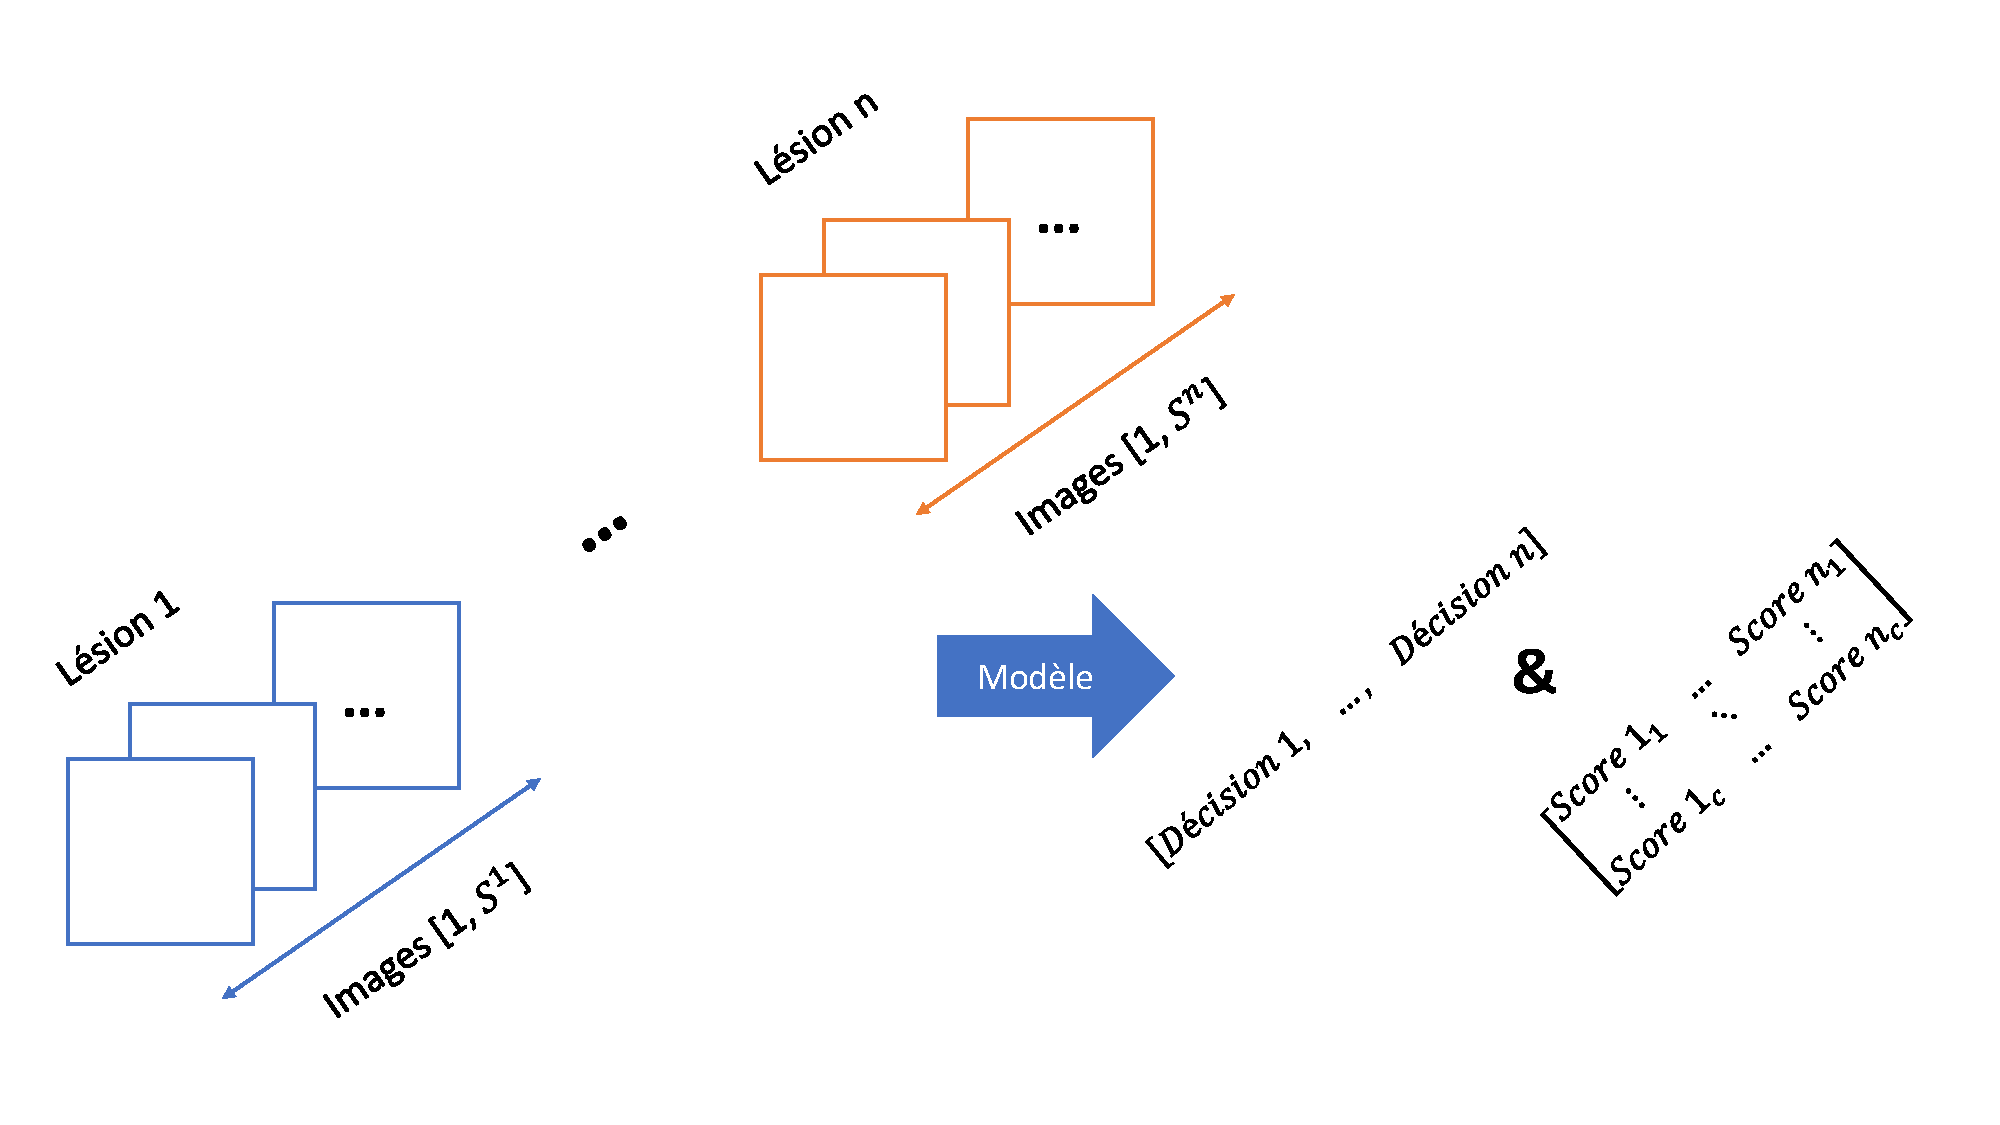
\includegraphics[width=0.75\linewidth]{contents/chapter_6/resources/scheme_patient_decision_objectives.pdf}
    \caption{Schéma récapitulatif de la problématique de l'inconsistance du nombres d'images constituant les lésions et de l'obtention de décisions et scores pour chacune de ces lésions.}
    \label{fig:scheme_patient_decision_objectives}
\end{figure}\par
\clearpage

\section{Approches supervisées}
Cette section dédiée aux approches supervisées se consacre à des schémas permettant de   l'aide d'annotation directes entre les données d'entrée et la sortie attendue. Les données \gls{rcm} exploitées dans ce travail possèdent :
\begin{inlinerate}
    \item d'une part des annotations à bas niveau ou niveau image,
    \item d'autre part des annotations à haut niveau ou niveau lésionnel. 
\end{inlinerate}. L'une des contraintes majeures associées à ces données est l'inconsistance du nombre d'images entre les lésions composant le jeu de données. Ainsi, une lésion peut comporter un nombre d'image compris entre une dizaine et une centaine d'entre elles. Il est donc nécessaire de gérer cette variabilité au sein du processus de classification mis en place.\par

Afin de résoudre cette tâche de manière supervisée, cette section propose un mécanisme de prédiction en deux temps : 
\begin{itemize}
    \item une première étape de prédiction dont le but consiste à évaluer la teneur des images,
    \item une seconde étape de prédiction au niveau des lésions dont la finalité est d'évaluer la lésion à partir de l'information résultant du processus de classification au niveau image.
\end{itemize} Dans ce but, les données d'entraînement sont divisées en deux parts, l'une d'entre elle à destination du processus de prédiction image et l'autre à destination du processus décisionnel des lésions. Cette séparation des données d'entraînement permet de contrer un sur-apprentissage du modèle de prédiction au niveau lésionnel par l'utilisation de données images pour lesquelles les prédictions seraient trop optimistes. Le schéma global mis en oeuvre dans cette section est disponible sur la \Cref{fig:scheme_patient_decision}.\par

\begin{figure}[H]
    \centering
    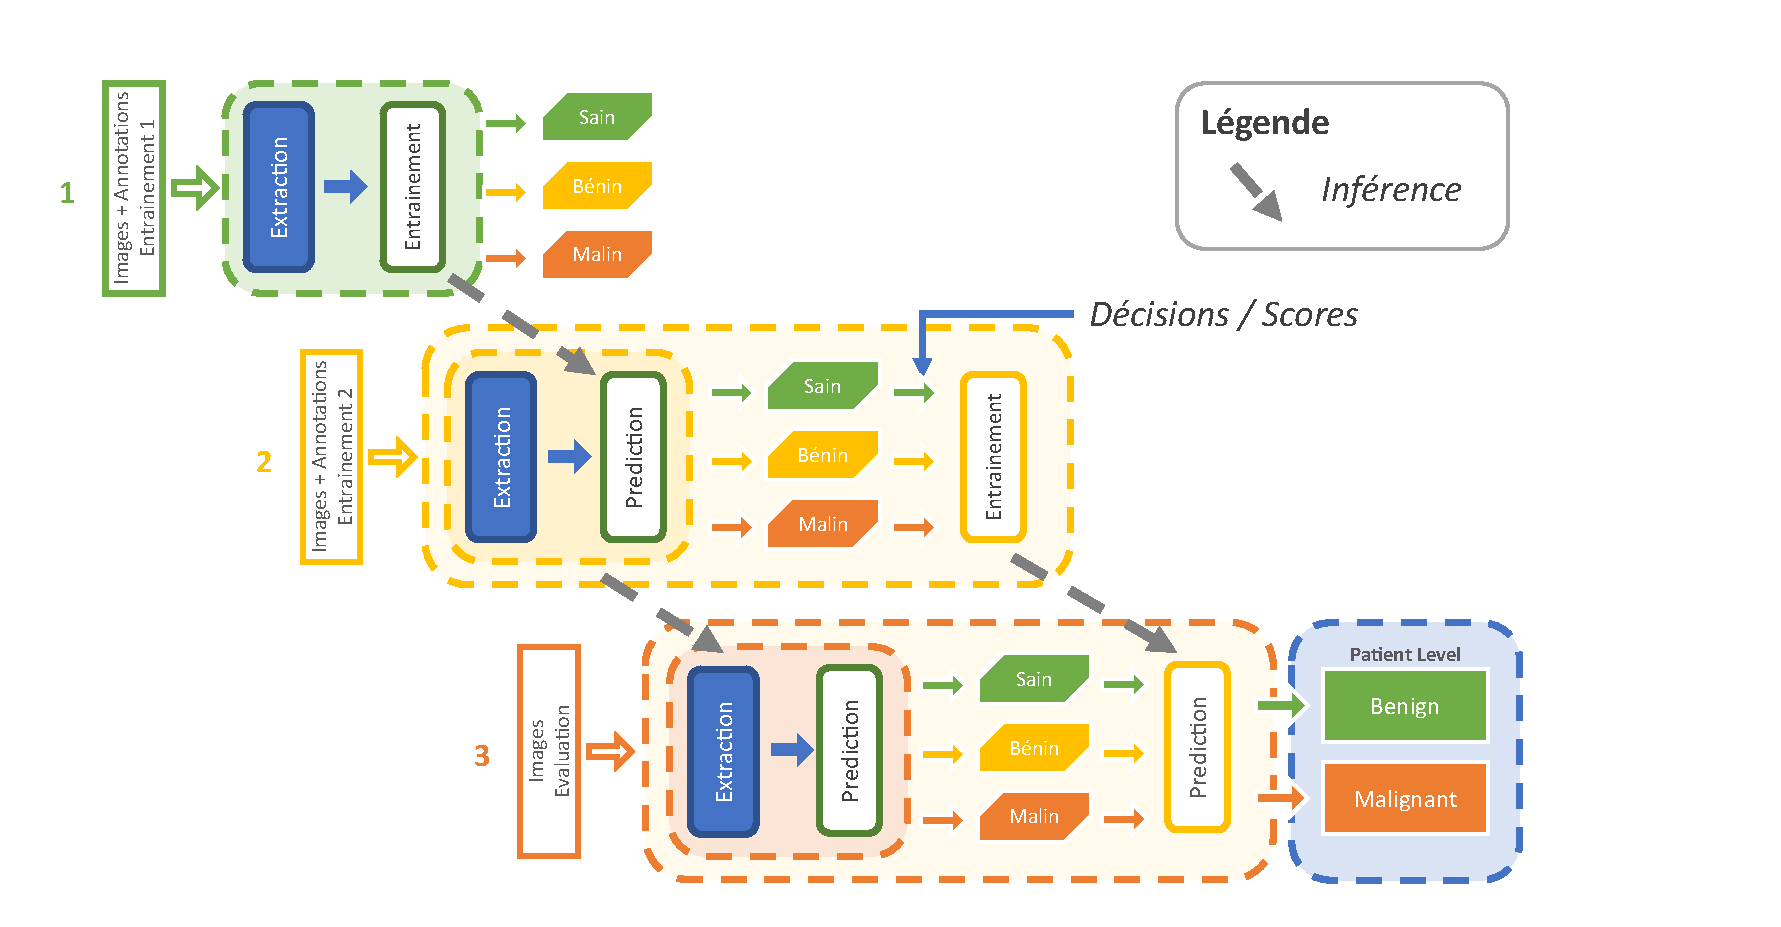
\includegraphics[width=\linewidth]{contents/chapter_6/resources/scheme_patient_decision.pdf}
    \caption{Schéma de représentation du système complet de décision supervisée au niveau lésionnel. Le processus d'entraînement se subdivise en deux étapes : une première étape d'entraînement du modèle de prédiction au niveau des instances images et une seconde étape permettant l'agrégation de l'information au niveau des lésions. La prédiction est ensuite réalisée sur les données de test par inférence des paramètres précédemment entraînés.}
    \label{fig:scheme_patient_decision}
\end{figure}\par

Ainsi, la première étape de prédiction exploite les conclusions issues des \Cref{chap:chapter_4,chap:chapter_5} dont le travail repose sur la prédiction au niveau image. Suite aux résultats de ces deux chapitres, cette première partie optera    \Cref{tab:parameters_lesion_classification_image_supervised}\par

\begin{table}[H]
    \centering
    \begin{tabular}{lll}
        \toprule
        \textbf{Modèle}                                 & \textbf{Hyperparamètres}  & \textbf{Valeurs}                          \\ \midrule
        \gls{svm} - Noyau linéaire                      & C                         & [0.001, 0.01, 0.1, 1, 10, 100, 1000]      \\ 
        \bottomrule 
    \end{tabular} 
    \caption{Table reprenant le modèle et les hyperparamètres du modèle de classification employé pour la détection bas niveau des images.}
    \label{tab:parameters_lesion_classification_image_supervised}
\end{table}\par

La seconde étape
\clearpage

\section{Approches faiblement supervisées}
Une approche est décrite comme étant faiblement supervisée lorsque l'apprentissage de la relation entre les données et les annotations n'est pas directe. Ainsi, ces méthodes faiblement supervisées sont rassemblées en trois catégories majeures~\cite{Zhou2018}, dont :
\begin{inlinerate}
    \item la \textbf{supervision dite incomplète} lorsque les données d'entraînement sont partiellement annotées,
    \item la \textbf{supervision dite inexacte} lorsque les annotations sont insuffisantes vis à vis du niveau de détails souhaité,
    \item et la \textbf{supervision dite imprécise} lorsque les annotations proviennent de sources manquant d'exactitude.
\end{inlinerate} Ces diverses approches ont notamment servies à la résolution de tâches telles que de la catégorisation de textes~\cite{Andrews2003,Settles2008} ou d'images~\cite{Chen2004,Tang2009}. Plus spécifiquement au domaine médical, ces techniques ont permis l'aide au diagnostic d'images médicales sur des pathologies pulmonaires ou du colon~\cite{Dundar2007} mais également du cancer du sein~\cite{Sudharshan2019}.\par

A cette fin, les annotations et les données images propres à chacune des lésions seront employées pour servir cette tâche faiblement supervisée. Par la nature des données en notre possession, cette nouvelle section s'intéresse au second mode de supervision dite inexacte, par l'utilisation de \textbf{méthodes à instances multiples}. De manière plus formelle ces techniques visent à résoudre la relation $f: X \mapsto Y$, à l'aide des données $D=\{(X_1,y_1),(X_2,y_2),\ldots,(X_b,y_b)\}$ avec $X=\{x_1,x_2,\ldots,x_b\}$ représentant un "sac" ou \textit{bag} d'information composé d'images et $y$ l'annotation associée~\cite{foulds2010}.\par

le compromis entre la solidité, l'exhaustivité et la convexité
Instance-based kernels
Set-based kernels
Hybrid approaches
sMIL
NSK
SIL
\gls{sil}
\cite{Andrews2002}

L'ensemble des modèles de prédiction exploitant le principe d'apprentissage par instances multiples que nous mettrons en oeuvre dans ce chapitre sont listés en \Cref{tab:patient_decision_weak_hyperparameters}. Afin de mener à bien la réalisation de ces expériences, nous nous reposerons essentiellement sur la librairie logicielle “MISVM” prévue à cet effet~\cite{Doran2014}.\par

\begin{table}[H]
    \centering
    \begin{tabular}{lll}
    \toprule
    \textbf{Méthode}    & \textbf{Paramètre}& \textbf{Valeurs}                                  \\ \midrule
    SIL                 & \multirow{3}{*}{C}& \multirow{3}{*}{[0.01, 0.1, 1, 10, 100, 1000]}    \\ \cline{1-1}
    mi-SVM              &                   &                                                   \\ \cline{1-1} 
    MI-SVM              &                   &                                                   \\ \bottomrule 
    \end{tabular}    
    \caption{Table reprenant les modèles faiblement supervisés pour attenter une classification au niveau lésionnel, ainsi que les hyperparamètres associés.}
    \label{tab:patient_decision_weak_hyperparameters}
\end{table}\par

\section{Analyse des résultats}
Dans cette section dédiée aux résultats, les diverses méthodes envisagées pour la prise de décision au niveau des lésions vont être traités à l'aide de paragraphes respectifs. Pour chaque méthode, les résultats de la classe maligne seront recueilli et les méthodes possédant le meilleur \fscore{} seront mise en avant. Ce premier paragraphe à destination des techniques supervisées va permettre de décrire les résultats obtenus par ces diverses méthodes. Ainsi, des différences significatives sont à remarquer entre les méthodes spatiales, fréquentielles et de transfert de connaissances, nettement à l'avantage de cette dernière méthode comme mise en avant lors du \Cref{chap:chapter_4}. Un \fscore{} maximum et stable de 0,88$\pm$0,04 est obtenu sur les classes malignes à l'aide de la méthode d'extraction par transfert de connaissances et par utilisation de la méthode de prise de décision à haut niveau par l'utilisation d'un seuil dynamique.\par

\begin{table}[H]
    \centering
    \begin{tabular}{cllll}
        \toprule
        \multicolumn{1}{l}{}         &                      & Précision          & Rappel             & \fscore{}            \\ \midrule
        \multirow{4}{*}{Spatial}     & Décisions - Priorité & \textbf{0.71±0.06} & \textbf{0.94±0.05} & \textbf{0.81±0.04} \\
                                     & Décisions - Dynamique& 0.77±0.10          & 0.78±0.10          & 0.77±0.05          \\
                                     & Scores - Maximum     & 0.69±0.10          & 0.83±0.19          & 0.75±0.06          \\
                                     & Scores - Moyenne     & 0.75±0.11          & 0.82±0.17          & 0.78±0.06          \\ \midrule
        \multirow{4}{*}{Fréquentiel} & Décisions - Priorité & 0.70±0.10          & 0.93±0.03          & 0.80±0.07          \\
                                     & Décisions - Dynamique& 0.81±0.06          & 0.79±0.05          & 0.80±0.02          \\
                                     & Scores - Maximum     & 0.72±0.09          & 0.78±0.25          & 0.75±0.13          \\
                                     & Scores - Moyenne     & \textbf{0.82±0.07} & \textbf{0.80±0.12} & \textbf{0.81±0.03} \\ \midrule
        \multirow{4}{*}{Transfert}   & Décisions - Priorité & 0.69±0.10          & 0.99±0.03          & 0.81±0.08          \\
                                     & Décisions - Dynamique& \textbf{0.84±0.07} & \textbf{0.92±0.07} & \textbf{0.88±0.04} \\
                                     & Scores - Maximum     & 0.79±0.09          & 0.93±0.05          & 0.85±0.05          \\
                                     & Scores - Moyenne     & 0.82±0.09          & 0.93±0.08          & 0.87±0.04          \\ \bottomrule
    \end{tabular}
    \caption{Résultats issus des processus de classification supervisés employés pour mener une classification au niveau lésionnel.}
    \label{tab:results_lesion_classification_supervised_patient}
\end{table}\par

\begin{table}[H]
    \centering
    \begin{tabular}{cllll}
        \toprule
        \multicolumn{1}{l}{}         &              & Précision          & Rappel             & \fscore{}            \\ \midrule
        \multirow{4}{*}{Spatial}     & SIL          & \textbf{0.67±0.14} & \textbf{0.95±0.05} & \textbf{0.79±0.11} \\
                                     & MI-SVM       & 0.75±0.07          & 0.67±0.09          & 0.71±0.08          \\
                                     & Scale SIL    & 0.68±0.09          & 0.97±0.02          & 0.80±0.06          \\
                                     & Scale MI-SVM & 0.86±0.06          & 0.78±0.01          & 0.82±0.03          \\ \midrule
        \multirow{4}{*}{Fréquentiel} & SIL          & 0.67±0.10          & 0.97±0.02          & 0.80±0.07          \\
                                     & MI-SVM       & 0.79±0.03          & 0.70±0.09          & 0.74±0.06          \\
                                     & Scale SIL    & 0.64±0.10          & 0.99±0.01          & 0.78±0.08          \\
                                     & Scale MI-SVM & \textbf{0.84±0.03} & \textbf{0.80±0.04} & \textbf{0.82±0.03} \\ \midrule
        \multirow{4}{*}{Transfert}   & SIL          & 0.69±0.10          & 0.99±0.01          & 0.82±0.07          \\
                                     & MI-SVM       & \textbf{0.86±0.06} & \textbf{0.83±0.10} & \textbf{0.85±0.06} \\
                                     & Scale SIL    & 0.69±0.10          & 1.00±0.00          & 0.81±0.08          \\
                                     & Scale MI-SVM & 0.87±0.06          & 0.88±0.03          & 0.87±0.04          \\ \bottomrule
    \end{tabular}
    \caption{Résultats issus des processus de classification faiblement supervisés employés pour mener une classification au niveau lésionnel.}
    \label{tab:results_lesion_classification_weakly_patient}
\end{table}\par

\begin{figure}[H]
    \centering
    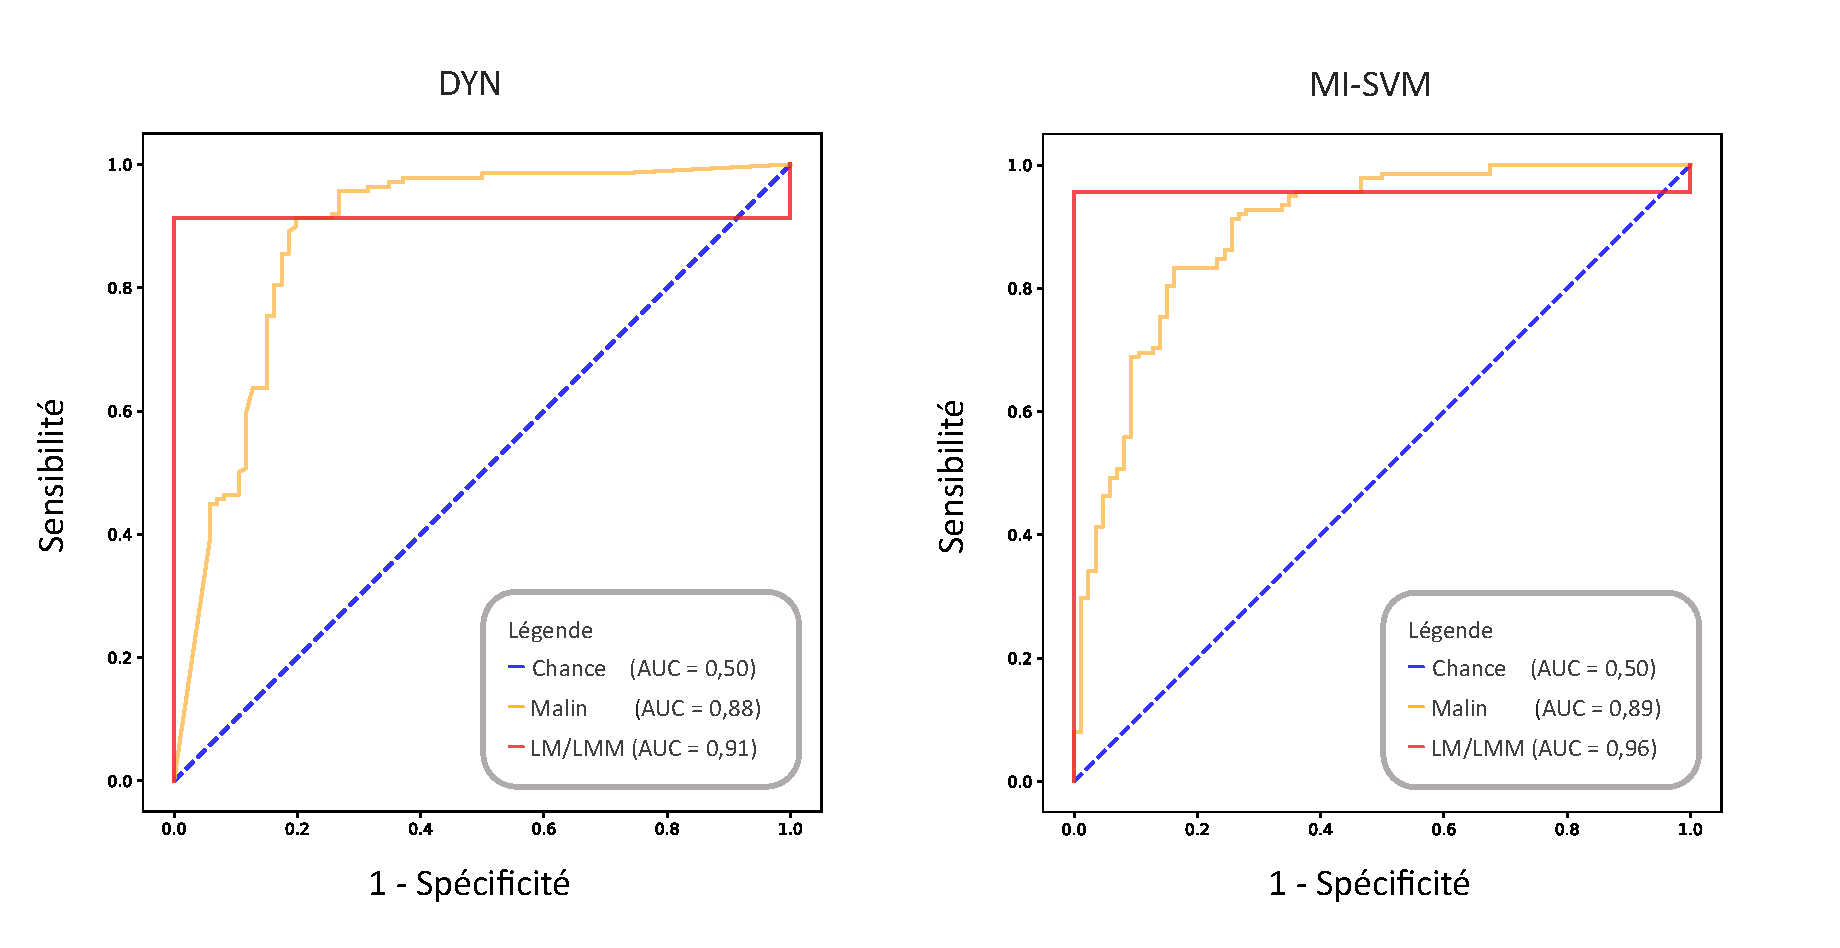
\includegraphics[width=\linewidth]{contents/chapter_6/resources/results_lesion_roc_lesions.pdf}
    \caption{Courbes \gls{roc} issus de la prédiction au niveau des lésions à partir d'entrainement de modèles de prédictions supportant ce niveau de prédiction. A gauche, les courbes issus du modèle de prédiction supervisé sur base de seuils dynamiques ; A droite, les courbes issus du modèle de prédiction MI-SVM.}
    \label{fig:results_lesion_roc_lesions}
\end{figure}\par

\begin{table}[H]
    \centering
    \begin{tabular}{cllll}
        \toprule
        \multicolumn{1}{l}{}         &              & Précision          & Rappel             & \fscore{}            \\ \midrule
        \multirow{4}{*}{Spatial}     & SIL          & 0.63±0.18          & 0.74±0.12          & 0.68±0.16          \\
                                     & MI-SVM       & 0.69±0.11          & 0.29±0.08          & 0.41±0.10          \\
                                     & MMS + SIL    & \textbf{0.72±0.09} & \textbf{0.80±0.08} & \textbf{0.76±0.08} \\
                                     & MMS + MI-SVM & 0.85±0.09          & 0.39±0.09          & 0.54±0.10          \\ \midrule
        \multirow{4}{*}{Fréquentiel} & SIL          & 0.67±0.15          & 0.80±0.06          & 0.73±0.12          \\
                                     & MI-SVM       & 0.81±0.07          & 0.26±0.07          & 0.39±0.08          \\
                                     & MMS + SIL    & \textbf{0.71±0.08} & \textbf{0.85±0.07} & \textbf{0.77±0.06} \\
                                     & MMS + MI-SVM & 0.89±0.04          & 0.43±0.12          & 0.58±0.11          \\ \midrule
        \multirow{4}{*}{Transfert}   & SIL          & \textbf{0.74±0.08} & \textbf{0.88±0.05} & \textbf{0.81±0.06} \\
                                     & MI-SVM       & 0.90±0.06          & 0.51±0.12          & 0.65±0.11          \\
                                     & MMS + SIL    & 0.73±0.09          & 0.85±0.05          & 0.79±0.06          \\
                                     & MMS + MI-SVM & 0.92±0.04          & 0.47±0.14          & 0.63±0.12          \\ \bottomrule
    \end{tabular}
    \caption{Résultats issus des processus de classification faiblement supervisés employés pour mener une classification au niveau des instances de cette problématique également considérée sous le nom d'images.}
    \label{tab:results_lesion_classification_weakly_image}
\end{table}\par

\begin{figure}[H]
    \centering
    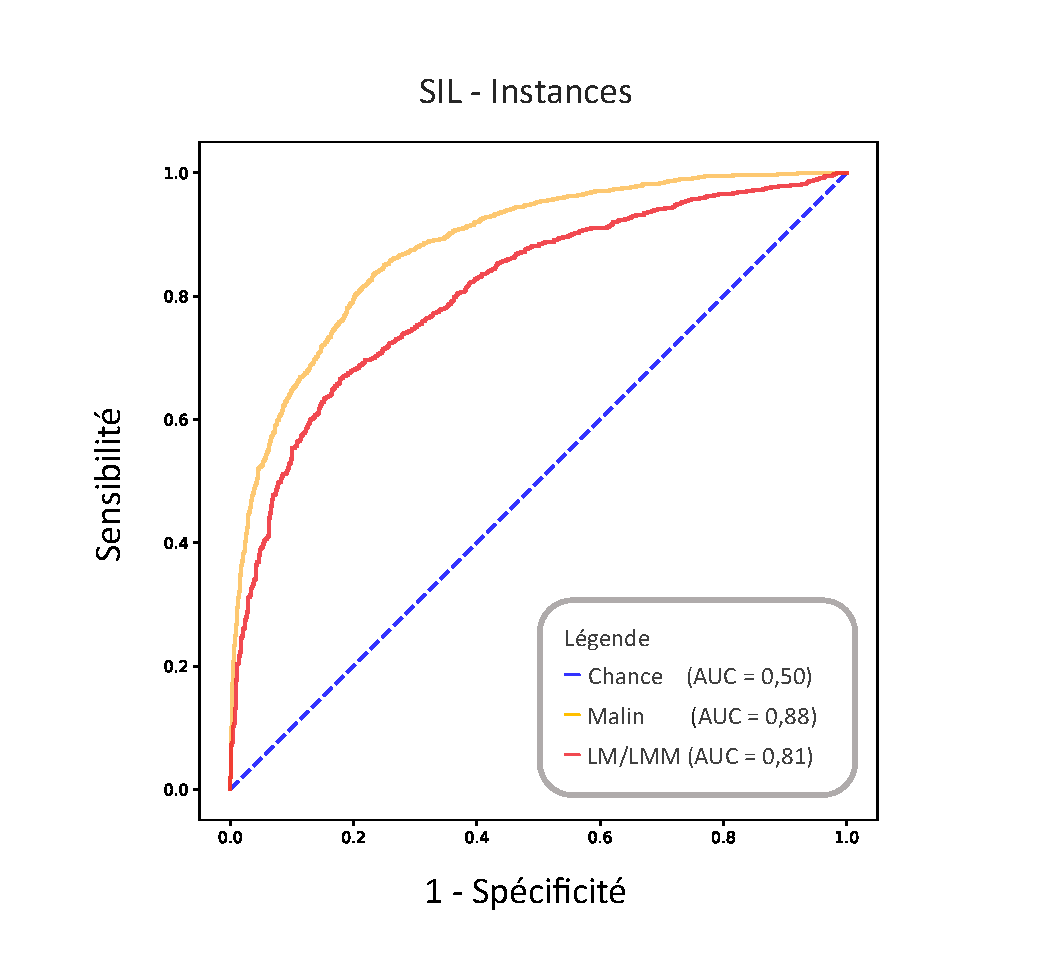
\includegraphics[width=\linewidth]{contents/chapter_6/resources/results_lesion_roc_instances.pdf}
    \caption{Courbes \gls{roc} issus de la prédiction au niveau des instances images à partir d'un entraînement faiblement supervisé employant les annotations des lésions pour qualifier un ensemble d'instances image.}
    \label{fig:results_lesion_roc_instances}
\end{figure}\par

\section{Discussion}
% This part relates to different ways to achieve classification at the patient-level based on the same two categories: “malignant”, as the positive class, and “benign”. With this assumption, a patient should be considered “malignant” if at least one image is considered to be “malignant”. Additionally, this part needs to consider the varying number of samples per patient (as a reminder, the number of instances per patient can vary between 2 and 833 images).\par
% In order to achieve this, the best combination of the feature extraction method and the classification model from \Cref{sec:image_decision} was used. The classification model provided two types of information for each image: the score was based on prediction probabilities and the decision (i.e., the class that achieved the best probability). In both cases, due to the varying number of images per patient, the information needs to be transformed into constant-size matrices to make a decision for existing and for new patients. At the score level, the structure was composed of patients, images, and scores of classes and transformed into a new matrix of size P*C, where P is the number of patients and C is the number of classes. A dynamic threshold was then used to adjust the positive class that maximizes the chosen metric. Multiple strategies can be used to achieve this:
% \begin{itemize}
% \item Mean - allows the contribution of each instance on the patient to be retained
% \item Maximum – retention of the best confidence prediction as to the trusted one.
% \end{itemize}
% \begin{figure}[H]
%     \begin{center}
%         \includegraphics[width=0.8\linewidth]{Figures/Process_Decision.pdf}
%         \caption{The classification process performed on \ac{rcm} patients in which the first part of the process remained the same as in \Cref{sec:image_decision}. The “Fit Model” and “Prediction” boxes refer to the decision and score level methods discussed in \Cref{sec:patient_decision}. The testing set was predicted for the patients based on “benign” and “malignant” classes.}
%         \label{fig:decision_process}
%     \end{center} 
% \end{figure}\par
% At the decision level, the structure was composed of structure, combining patients, images, and scores of classes and transformed into a new matrix of size P*C, where P is the number of patients and C is the number of classes. Also, C refers to the probability vector of each decision between 0 and 1.
% \begin{itemize}
% \item At Least One - at least one positive decision to consider the input as positive (initial assumption)
% \item Dynamic - find a dynamic threshold that minimizes false-positive decisions.
% \end{itemize}
% A global overview of the processing scheme of this method is presented in \Cref{fig:decision_process}.
% In a second stage, a number of \ac{mil} concepts are implemented in this part, as they fit the issue at hand: a patient is constitutive of several instances (consider it as a bag) and a positive instance assumes that the patient should be positive. Furthermore, only the patient label is known, and the annotation step of individual images is time-consuming. Such a problem can be set as a pair\(\{X|y\}\), in which \(X=\{X^1,X^2,\ldots,X^b\}\) is a bag containing \(b\) instances and each \(X^b\) formulated as follows: \(X^b=\{x^b_1,x^b_2,\ldots,x^b_n\}\), in which \(n\) is the number of features and \(y\) is the patient label~\cite{foulds_frank_2010}. Two ideas are developed regarding this context in the paragraphs that follow. In a first stage, a \ac{sil} classification is used in which a bag is considered as negative if all of the instances are considered to be negative, and positive if at least one of the instances has a positive label that fits our initial formulation of the patient label. In a second stage, the MI-SVM is an extension of \ac{svm} upon \ac{mil} theory and is employed in these due to the results of \Cref{sec:image_decision}. These experiments are configured to function with a linear kernel due to the observation made by the experiments of \Cref{sec:image_decision}. In this part, the experiments were implemented using the “MISVM” library~\cite{Doran2014}.\par
% In addition, to provide the best performance on each of these models, a search for their optimal hyper-parameters was carried out (see \Cref{tab:patient_hyperparameters}).\par


% The validation protocol remains the same for each of these experiments, based on a nested cross-validation that is known to be less biased than a simple cross-validation scheme~\cite{Cawley2010}. This protocol allows 1) cross-validation of hyper-parameters and 2) objective evaluation of the prediction models. Each of the cross-validation step is based on a K-fold strategy with a $k$ value of 4 on the testing loop and 2 on the validation loop. Also, each time, the patients are separated and balanced as best as possible based on the image labels. In order to achieve an objective evaluation, each data cluster remains the same for the experiments in a given section (refer to \Cref{sec:image_decision} and \Cref{sec:patient_decision}). Moreover, each experiment is validated and evaluated using a \fscore{} metric, as it is statistically suitable for unbalanced populations in comparison with accuracy, and it represents in a single value both recall and precision information. In addition, standard deviation is computed to analyse the stability of models along the nested cross-validation. For this purpose, we used the “Scikit Learn” library for Machine Learning classification, validation, and metric~\cite{pedregosa2011scikit}.\par


% This paragraph focuses on the methods implemented to reach the patient diagnosis (see \Cref{sec:patient_decision}) and it relates to the initial \ac{rcm} data (including unlabeled images) used previously to evaluate specialists~\cite{Cinotti2018}. All these experimental results are listed in \Cref{tab:patient_results} and discussed below. Firstly, the methods performance varied between 0.61 and 0.84 in terms of the \fscore{} for Malignancy. The “At Least One” method achieved poor performance due to prediction errors over the “benign” class. This problem can be solved by the use of a dynamic activation threshold for decisions to minimize the risk of false-positives, at the cost of resulting in an ethical consideration of this method in the clinical context. Secondly, the methods based on the score are almost the same and varied from 0.76 to 0.83 for the \fscore{} for Malignancy. By contrast, with these results, the standard deviations remained reasonable, varying from 0.03 to 0.06. Finally, \ac{mil} was also evaluated, and a substantial difference was noted between the \ac{sil} and the MI-SVM. Indeed, the \ac{sil} assumption yielded similar results with the decision based on the “At Least One” method, due to an insufficient ability to discriminate on the same “benign” class. By contrast, the MI-SVM yielded a number of good results, with an \fscore{} of 0.82. Both methods are stable, with a deviation that only varied from 0.02 to 0.04. Poor results with the “At Least One” and the \ac{sil} methods can be due to a lack of discriminative information provided by the “Inception-ResNet” for these methods.\par
% \begin{table}[H]
%     \centering
%     \begin{tabular}{lllll}
%                                 &                   & \multicolumn{3}{c}{\textbf{Malignancy - \fscore{}}}                    \\ \hline
%     \textbf{Category}           & \textbf{Name}     & \textbf{Weighted}     & \textbf{Benign}       & \textbf{Malignant}    \\ \hline
%     \multirow{2}{*}{Decision}   & At Least One      & 0.61$\pm$0.06         & 0.32$\pm$0.07         & 0.79$\pm$0.05         \\ \cline{2-5} 
%                                 & \textbf{Dynamic}  & \textbf{0.84$\pm$0.03}& \textbf{0.78$\pm$0.07}& \textbf{0.87$\pm$0.02}\\ \hline 
%     \multirow{2}{*}{Score}      & Mean              & 0.83$\pm$0.03         & 0.78$\pm$0.08         & 0.87$\pm$0.02         \\ \cline{2-5}
%                                 & Maximum           & 0.76$\pm$0.04         & 0.68$\pm$0.03         & 0.80$\pm$0.05         \\ \hline  
%     \multirow{2}{*}{\ac{mil}}   & \ac{sil}          & 0.70$\pm$0.04         & 0.50$\pm$0.10         & 0.83$\pm$0.03         \\ \cline{2-5} 
%                                 & \textbf{MI-SVM}   & \textbf{0.82$\pm$0.02}& \textbf{0.78$\pm$0.05}& \textbf{0.84$\pm$0.02}\\ \hline 
%     \end{tabular}    
%     \caption{Results for the patient-level classification for Malignancy (\ac{lm} and \ac{bcc}) according to the different methods from \Cref{sec:patient_decision}. For Malignancy and \ac{lm}, the table provides a weighted average \fscore{} and individual \fscore{} for the benign and the malignant classes.}
%     \label{tab:patient_results}
% \end{table}\par
% Following previous results, this paragraph discusses in detail the results of supervised “Dynamic” decision threshold and \ac{mil} based on “MI-SVM” methods over the Malignancy (meaning \ac{bcc} and \ac{lm}) and \ac{lm} as the cited clinical study does~\cite{Cinotti2018}. \Cref{tab:patient_results_details} provides \fscore{}, precision, and recall based on these experiments. As the classification is binary, recall of the positive class refers to the sensitivity and recall of the negative class refers to the Specificity. The “Dynamic” method achieves scores of 0.89$\pm$0.03 sensitivity and 0.75$\pm$0.07 specificity for Malignancy; 0.88$\pm$0.04 sensitivity and 0.75$\pm$0.07 specificity for \ac{lm} pathologies. The “MI-SVM” method achieves scores of 0.80$\pm$0.02 sensitivity and 0.84$\pm$0.05 specificity for Malignancy; 0.78$\pm$0.07 sensitivity and 0.84$\pm$0.07 specificity for \ac{lm} pathologies. The “Dynamic” method provides more emphasis on sensitivity while “MI-SVM” provides a good specificity. These methods are quite comparable to the evaluation of the dermatologists, reaching 0.80 of sensitivity and 0.81 of specificity, but less homogeneous compared to them.\par
% \par
% \begin{table}[H]
%     \centering
%     \begin{tabular}{lllll||lll}
%                                 &                   & \multicolumn{3}{c}{\textbf{Malignancy}}                               & \multicolumn{3}{c}{\textbf{\ac{lm}}}                                  \\ \hline
%     \textbf{Name}               & \textbf{Label}    & \textbf{\fscore{}}     & \textbf{Precision}    & \textbf{Recall}       & \textbf{\fscore{}}     & \textbf{Precision}    & \textbf{Recall}       \\ \hline
%     \multirow{3}{*}{Dynamic}    & Benign            & 0.78$\pm$0.07         & 0.81$\pm$0.08         & 0.75$\pm$0.07         & 0.79$\pm$0.06         & 0.82$\pm$0.07         & 0.75$\pm$0.07         \\ \cline{2-8}  
%                                 & Malignant         & 0.87$\pm$0.02         & 0.85$\pm$0.03         & 0.89$\pm$0.03         & 0.86$\pm$0.03         & 0.83$\pm$0.03         & 0.88$\pm$0.04         \\ \cline{2-8} 
%                                 & Weighted          & 0.84$\pm$0.03         & 0.84$\pm$0.03         & 0.84$\pm$0.03         & 0.83$\pm$0.03         & 0.83$\pm$0.03         & 0.83$\pm$0.03         \\ \hline
%     \multirow{3}{*}{MI-SVM}     & Benign            & 0.78$\pm$0.02         & 0.72$\pm$0.08         & 0.84$\pm$0.07         & 0.78$\pm$0.05         & 0.73$\pm$0.07         & 0.84$\pm$0.07         \\ \cline{2-8}
%                                 & Malignant         & 0.84$\pm$0.02         & 0.89$\pm$0.05         & 0.80$\pm$0.05         & 0.82$\pm$0.03         & 0.87$\pm$0.06         & 0.78$\pm$0.07         \\ \cline{2-8} 
%                                 & Weighted          & 0.82$\pm$0.02         & 0.82$\pm$0.02         & 0.83$\pm$0.02         & 0.80$\pm$0.03         & 0.80$\pm$0.03         & 0.81$\pm$0.02         \\ \hline 
%     \end{tabular}    
%     \caption{Detailed results for the patient-level classification for the Decision method based on a Dynamic threshold and \ac{mil} based on the MI-SVM assumption. The table provides the \fscore{}, Precision, and Recall for the benign and malignant classes with these methods.}
%     \label{tab:patient_results_details}
% \end{table}\par
% Finally, \Cref{fig:roc_results} provides \ac{roc} curves for both malignancy and \ac{lm} pathologies on “Dynamic” and “MI-SVM” methods. In the context of Malignancy evaluation, the measured \ac{auc} is 0.89 for “MI-SVM” and 0.88 for “Dynamic”. For \ac{lm} evaluation, the measured \ac{auc} is 0.88 for “MI-SVM” and 0.87 for “Dynamic”. In the same context of \ac{lm} lesions, the experts obtained an \ac{auc} score of 0.89, so close to the previous two methods. Apart from this, \Cref{fig:misclassified} provides some misleading images: the \ac{rcm} images in the center belongs to the same patient (image c and d) with similar patterns and homogeneous information while the \ac{rcm} images on the outside parts of the figure contain hair, artifacts, tricky patterns or nonhomogeneous information (image a, b, e, and f). Also, the images on the bottom left and the bottom right (image b and e) of the figure are examples of images were experts will use stacks of images to make their decision and where the currently developed methods only use a single image.
% \begin{figure}[H]
%     \centering
%     \begin{subfigure}{0.47\linewidth}
%         \centering
%         \textbf{Malignancy \ac{roc} curves}\par
%         \includegraphics[width=\linewidth]{Figures/Result_Malignancy.pdf}
%     \end{subfigure}
%     \begin{subfigure}{0.47\linewidth}
%         \centering
%         \textbf{\ac{lm} \ac{roc} curves}\par
%         \includegraphics[width=\linewidth]{Figures/Result_LMM.pdf}
%     \end{subfigure} 
%     \caption{On the left, the \ac{roc} curves for Malignancy with the Dynamic and MI-SVM methods. On the right, the \ac{roc} curves for \ac{lm} with the Dynamic and MI-SVM methods.}
%     \label{fig:roc_results}
% \end{figure}

% \begin{figure}[H]
%     \centering
%     \includegraphics[width=\linewidth]{Figures/Misclassified.pdf}
%     \caption{Examples of \ac{rcm} images that mislead the classifier with the highest \fscore{} (Inception-ResNet + SVM - Linear). On the left part (image a, b and c), \ac{rcm} images belonging to the benign label and classified as malignant. On the right part (image d, e and f), \ac{rcm} images belonging to the malignant label and classified as benign. In the center of the figure (image c and d), two \ac{rcm} images of the same patient belonging to benign and malignant labels.}
%     \label{fig:misclassified}
% \end{figure}